\documentclass[10pt]{beamer}

% Copia local de preamble.tex:
\usetheme[progressbar=frametitle]{metropolis}
\usepackage{appendixnumberbeamer}
\usepackage{fancyvrb}
\usepackage{booktabs}
\usepackage[scale=2]{ccicons}
\usepackage{pgfplots}
\usepgfplotslibrary{dateplot}
\usepackage{type1cm}
\usepackage{lettrine}
\usepackage{ragged2e}
\usepackage{xspace}
\newcommand{\themename}{\textbf{\textsc{metropolis}}\xspace}
\usepackage{graphicx} % Allows including images
\usepackage{booktabs} % Allows the use of \toprule, \midrule and \bottomrule in tables
\usepackage[utf8]{inputenc} %solucion del problema de los acentos.
\usepackage{xcolor}
\definecolor{LightGray}{gray}{0.9}

\usepackage{minted}
\usemintedstyle{tango}
\newcommand{\mypyfile}[1]{\inputminted[linenos=true, fontsize=\footnotesize, frame=lines, framesep=5\fboxrule,framerule=1pt]{python}{#1}}

\setminted[python]{breaklines,frame=lines,framesep=2mm,baselinestretch=1.2,bgcolor=LightGray,linenos, fontsize=\footnotesize} % obeytabs=true, tabsize=2, showtabs=true}

%%%%%%%%%%%%%%%%%%%%%%%%%%%%%%%%%%%%%%%%%%%%%%%%%%%%%%%%%%%%%%%%%%%%%%%%%%%%%%%%%%%%%%
\setbeamercolor{progress bar}{fg=blue!50!black,bg=white!50!black}
\setbeamercolor{title separator}{fg=red!50!black,bg=white!50!black}
\setbeamercolor{frametitle}{fg=white!80!black,bg=red!50!black}
\title[PCFI161]{Programaci\'on para F\'isica y Astronom\'ia}
\subtitle{Departamento de Física.}

\newcommand{\myfront}{
\author[PCFI161]{Corodinadora: C Loyola \\ Profesoras/es C Loyola / C Femenías / Y Navarrete / C Ruiz}
\institute[UNAB]{Universidad Andrés Bello}
\date{Primer Semestre 2025}
}

\titlegraphic{%
  
\includegraphics[width=.08\textwidth]{logo-tux.png}\hfill
  
\includegraphics[width=.3\textwidth]{logo-unab.png}\hfill
  
\includegraphics[width=.08\textwidth]{logo-python.png}
}

\makeatletter
\setbeamertemplate{title page}{
  \begin{minipage}[b][\paperheight]{\textwidth}
    \vfill%
    \ifx\inserttitle\@empty\else\usebeamertemplate*{title}\fi
    \ifx\insertsubtitle\@empty\else\usebeamertemplate*{subtitle}\fi
    \usebeamertemplate*{title separator}
    \ifx\beamer@shortauthor\@empty\else\usebeamertemplate*{author}\fi
    \ifx\insertdate\@empty\else\usebeamertemplate*{date}\fi
    \ifx\insertinstitute\@empty\else\usebeamertemplate*{institute}\fi
    \vfill
    \ifx\inserttitlegraphic\@empty\else\inserttitlegraphic\fi
    \vspace*{1cm}
  \end{minipage}
}
\makeatother


\makeatletter
\setlength{\metropolis@titleseparator@linewidth}{2pt}
\setlength{\metropolis@progressonsectionpage@linewidth}{2pt}
\setlength{\metropolis@progressinheadfoot@linewidth}{2pt}
\makeatother


\begin{document}

% Portada
\myfront{}

\begin{frame}
  \titlepage
\end{frame}

\begin{frame}
  \frametitle{Resumen}
  \tableofcontents
\end{frame}

%----------------------------------------------------------------------------------------
%	PRESENTATION SLIDES
%----------------------------------------------------------------------------------------

\metroset{block=fill}

%------------------------------------------------
\section{Computadores y Programaci\'on}
\subsection{Introducci\'on}

\begin{frame}{La m\'aquina Universal}
	\begin{itemize}
		\item Casi todos han usado un computador en alguna ocasi\'on, para jugar, escribir,  
		administrar el dinero, etc.
		\item Los computadores se usan para predecir clima, dise\~nar aviones, crear pel\'iculas, 
		hacer negocios, entre muchas otras cosas.
		\item ?`Pero qu\'e es un computador? ?`Por qu\'e puede realizar distintas tareas?.
		\item Un computador moderno podr\'ia definirse como una m\'aquina que almacena y manipula 
		informaci\'on bajo el control de un programa cambiable.
	\end{itemize}
\end{frame}

\begin{frame}{La M\'aquina Universal}
	\begin{itemize}
		\item Almacena y manipula:
		\begin{itemize}
			\item Transforma informaci\'on en otra informaci\'on \'util.
			\item Como una calculadora, operando con cientos o miles de n\'umeros.
			\item Como una m\'aquina para surtir gasolina (tarea espec\'ifica).
		\end{itemize}
		\item Operan bajo el control de un programa cambiable.
		\begin{itemize}
			\item Un programa es un set de instrucciones que le dice al computador exactamente lo 
			que debe hacer.
			\item Si el programa cambia, el computador realiza acciones distintas, y la tarea resultante
			tambi\'en es distinta.
		\end{itemize}
	\end{itemize}
\end{frame}

\begin{frame}{Programaci\'on}
	\begin{itemize}
		\item El \textit{Software} controla el \textit{Hardware}.
		\item Es el \textit{Software} el que determina lo que puede hacer el computador.
		\item Programar es una actividad desafiante, pero todos pueden aprender lo b\'asico.
	\end{itemize}
\end{frame}

\begin{frame}{Computer Science}
	\begin{itemize}\small
		\item Aprender \textit{Computer Science} no es solo estudiar computadores.
		\item Edsger Dijkstra: “los computadores son a Computer Science lo que los telescopios son a la astronomía”.
		\item Dise\~no, an\'alisis y experimentaci\'on son fundamentales para entender cu\'ales problemas
		      podemos (o no) resolver computacionalmente.
	\end{itemize}
\end{frame}

\begin{frame}{Hardware}
	\begin{itemize}\small
		\item CPU (Central Processing Unit): realiza operaciones b\'asicas.
		\item RAM (Random Access Memory): almacena programas y datos que la CPU est\'a usando.
		\item Almac\'en permanente (discos duros, memorias flash, etc.).
	\end{itemize}
\end{frame}

\begin{frame}{Wake up}
    \begin{block}{¿Qu\'e ocurre cuando ejecutamos un programa?}
		\begin{enumerate}\small
		\item Las instrucciones se copian desde el disco a la RAM.
		\item La CPU comienza a ejecutar esas instrucciones.
		\item Se sigue el ciclo \textit{fetch-execute}.
	    \end{enumerate}
	\end{block}
\end{frame}

\begin{frame}{Clusters de Computadores}
\begin{itemize}\small
    \item Un \textbf{clúster} es un conjunto de computadores que trabajan en paralelo para una tarea.
    \item Común en bancos, gobiernos, big data, desarrollo de IA, ciencia, etc.
\end{itemize}
\end{frame}

\begin{frame}[fragile]{Cluster grupo de materiales/Ejemplo de supercomputador}
 \begin{itemize}\scriptsize
	\item 19 Nodos de cómputo de CPU (44 Core cada uno)
    \item 4 Nodos GPU (Tesla K80)
    \item Switch IB+(2xRJ45)
    \item Nodos de acceso y disco
\end{itemize}

\begin{figure}
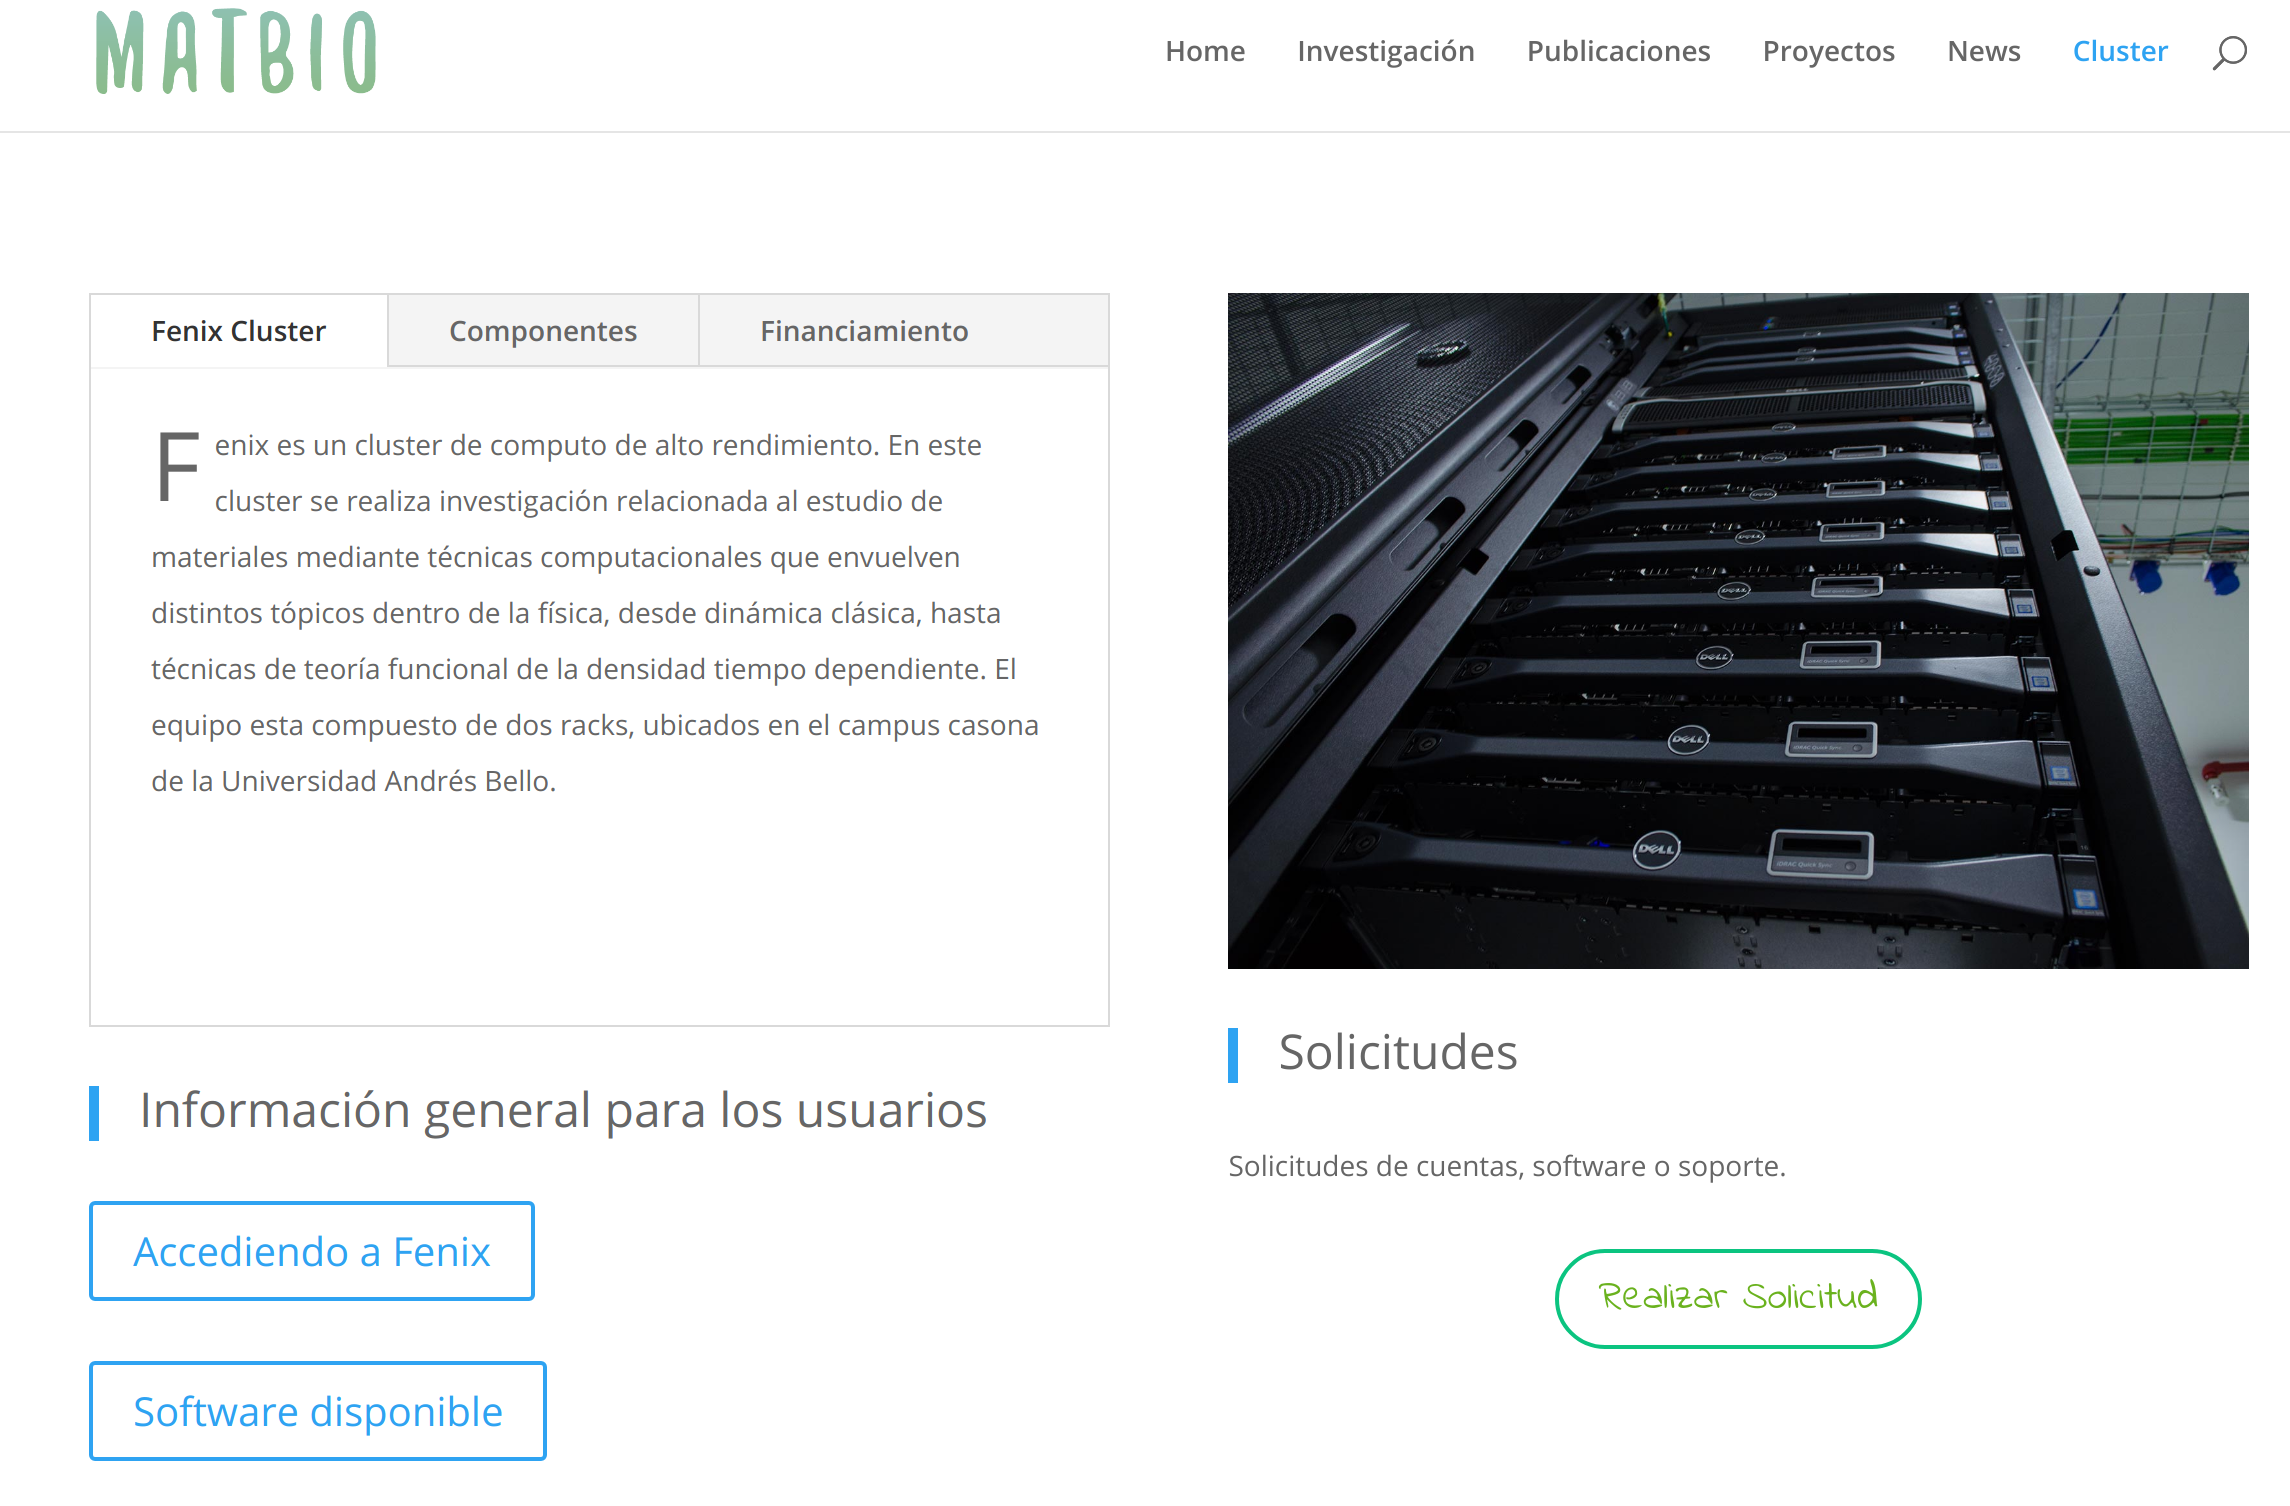
\includegraphics[width=0.6\textwidth]{homecluster}
\end{figure}
\end{frame}

%------------------------------------------------
% EJEMPLO / ACTIVIDAD ADICIONAL
%------------------------------------------------
\begin{frame}{Actividad Sugerida: Explorando tu propio computador}
\begin{itemize}
    \item \textbf{Objetivo:} Identificar los componentes de tu equipo y sus características básicas.
    \item \textbf{Instrucciones:}
    \begin{enumerate}
        \item Si usas Windows, revisa el “Administrador de tareas” (o “Task Manager”) para ver uso de CPU y RAM.
        \item Si usas GNU/Linux, ejecuta \texttt{lscpu}, \texttt{free -h} y \texttt{lsblk} para ver detalles de CPU, memoria y discos.
        \item Reflexiona: ¿qué pasa si abres muchos programas? ¿Cómo cambia el uso de la RAM y CPU?
    \end{enumerate}
    \item \textbf{Conclusión:} Comprender la interacción de CPU, RAM y almacenamiento.
\end{itemize}
\end{frame}

\begin{frame}
\Huge{\centerline{Fin de la Parte 1}}
\end{frame}

\end{document}

